%  LaTeX support: latex@mdpi.com
%  In case you need support, please attach all files that are necessary for compiling as well as the log file, and specify the details of your LaTeX setup (which operating system and LaTeX version / tools you are using).

%=================================================================
\documentclass[smartcities,article,submit,moreauthors,pdftex]{Definitions/mdpi}

% If you would like to post an early version of this manuscript as a preprint, you may use preprint as the journal and change 'submit' to 'accept'. The document class line would be, e.g., \documentclass[preprints,article,accept,moreauthors,pdftex]{mdpi}. This is especially recommended for submission to arXiv, where line numbers should be removed before posting. For preprints.org, the editorial staff will make this change immediately prior to posting.

%--------------------
% Class Options:
%--------------------
%----------
% journal
%----------
% Choose between the following MDPI journals:
% acoustics, actuators, addictions, admsci, aerospace, agriculture, agriengineering, agronomy, algorithms, animals, antibiotics, antibodies, antioxidants, applsci, arts, asc, asi, atmosphere, atoms, axioms, batteries, bdcc, behavsci , beverages, bioengineering, biology, biomedicines, biomimetics, biomolecules, biosensors, brainsci , buildings, cancers, carbon , catalysts, cells, ceramics, challenges, chemengineering, chemistry, chemosensors, children, cleantechnol, climate, clockssleep, cmd, coatings, colloids, computation, computers, condensedmatter, cosmetics, cryptography, crystals, dairy, data, dentistry, designs , diagnostics, diseases, diversity, drones, econometrics, economies, education, ejihpe, electrochem, electronics, energies, entropy, environments, epigenomes, est, fermentation, fibers, fire, fishes, fluids, foods, forecasting, forests, fractalfract, futureinternet, futurephys, galaxies, games, gastrointestdisord, gels, genealogy, genes, geohazards, geosciences, geriatrics, hazardousmatters, healthcare, heritage, highthroughput, horticulturae, humanities, hydrology, ijerph, ijfs, ijgi, ijms, ijns, ijtpp, informatics, information, infrastructures, inorganics, insects, instruments, inventions, iot, j, jcdd, jcm, jcp, jcs, jdb, jfb, jfmk, jimaging, jintelligence, jlpea, jmmp, jmse, jnt, jof, joitmc, jpm, jrfm, jsan, land, languages, laws, life, literature, logistics, lubricants, machines, magnetochemistry, make, marinedrugs, materials, mathematics, mca, medicina, medicines, medsci, membranes, metabolites, metals, microarrays, micromachines, microorganisms, minerals, modelling, molbank, molecules, mps, mti, nanomaterials, ncrna, neuroglia, nitrogen, notspecified, nutrients, ohbm, optics, particles, pathogens, pharmaceuticals, pharmaceutics, pharmacy, philosophies, photonics, physics, plants, plasma, polymers, polysaccharides, preprints , proceedings, processes, proteomes, psych, publications, quantumrep, quaternary, qubs, reactions, recycling, religions, remotesensing, reports, resources, risks, robotics, safety, sci, scipharm, sensors, separations, sexes, signals, sinusitis, smartcities, sna, societies, socsci, soilsystems, sports, standards, stats, surfaces, surgeries, sustainability, symmetry, systems, technologies, test, toxics, toxins, tropicalmed, universe, urbansci, vaccines, vehicles, vetsci, vibration, viruses, vision, water, wem, wevj

%---------
% article
%---------
% The default type of manuscript is "article", but can be replaced by:
% abstract, addendum, article, benchmark, book, bookreview, briefreport, casereport, changes, comment, commentary, communication, conceptpaper, conferenceproceedings, correction, conferencereport, expressionofconcern, extendedabstract, meetingreport, creative, datadescriptor, discussion, editorial, essay, erratum, hypothesis, interestingimages, letter, meetingreport, newbookreceived, obituary, opinion, projectreport, reply, retraction, review, perspective, protocol, shortnote, supfile, technicalnote, viewpoint
% supfile = supplementary materials

%----------
% submit
%----------
% The class option "submit" will be changed to "accept" by the Editorial Office when the paper is accepted. This will only make changes to the frontpage (e.g., the logo of the journal will get visible), the headings, and the copyright information. Also, line numbering will be removed. Journal info and pagination for accepted papers will also be assigned by the Editorial Office.

%------------------
% moreauthors
%------------------
% If there is only one author the class option oneauthor should be used. Otherwise use the class option moreauthors.

%---------
% pdftex
%---------
% The option pdftex is for use with pdfLaTeX. If eps figures are used, remove the option pdftex and use LaTeX and dvi2pdf.

%=================================================================
\firstpage{1}
\makeatletter
\setcounter{page}{\@firstpage}
\makeatother
\pubvolume{xx}
\issuenum{1}
\articlenumber{5}
\pubyear{2020}
\copyrightyear{2020}
%\externaleditor{Academic Editor: name}
\history{Received: date; Accepted: date; Published: date}
%\updates{yes} % If there is an update available, un-comment this line

%% MDPI internal command: uncomment if new journal that already uses continuous page numbers
%\continuouspages{yes}

%------------------------------------------------------------------
% The following line should be uncommented if the LaTeX file is uploaded to arXiv.org
%\pdfoutput=1

%=================================================================
% Add packages and commands here. The following packages are loaded in our class file: fontenc, calc, indentfirst, fancyhdr, graphicx, lastpage, ifthen, lineno, float, amsmath, setspace, enumitem, mathpazo, booktabs, titlesec, etoolbox, amsthm, hyphenat, natbib, hyperref, footmisc, geometry, caption, url, mdframed, tabto, soul, multirow, microtype, tikz

%=================================================================
%% Please use the following mathematics environments: Theorem, Lemma, Corollary, Proposition, Characterization, Property, Problem, Example, ExamplesandDefinitions, Hypothesis, Remark, Definition, Notation, Assumption
%% For proofs, please use the proof environment (the amsthm package is loaded by the MDPI class).

%=================================================================
% Full title of the paper (Capitalized)
\Title{Rider Perceptions of an On-Demand Microtransit Service in Salt Lake County, Utah}

% Author Orchid ID: enter ID or remove command
\newcommand{\orcidauthorA}{0000-0003-3999-7584} % Add \orcidA{} behind the author's name
%\newcommand{\orcidauthorB}{0000-0000-000-000X} % Add \orcidB{} behind the author's name

% Authors, for the paper (add full first names)
\Author{Gregory S. Macfarlane$^{1*}$\orcidA{}, Christian Hunter$^{1}$, Austin Martinez$^{1}$, and Elizabeth Smith$^{1}$}

% Authors, for metadata in PDF
\AuthorNames{Gregory S. Macfarlane, Christian Hunter, Austin Martinez, and Elizabeth Smith}

% Affiliations / Addresses (Add [1] after \address if there is only one affiliation.)
\address[1]{%
$^{1}$ \quad Department of Civil and Environmental Engineering, Brigham Young University}

% Contact information of the corresponding author
\corres{Correspondence: gregmacfarlane@byu.edu; Tel.: +01-801-422-8505}

% Current address and/or shared authorship
\firstnote{Current affiliation: University of Texas, Austin}
\secondnote{Current affiliation: Imperial College London}
% The commands \thirdnote{} till \eighthnote{} are available for further notes

%\simplesumm{} % Simple summary

%\conference{} % An extended version of a conference paper

% Abstract (Do not insert blank lines, i.e. \\)
\abstract{On-demand microtransit services are frequently seen as an important tool in supporting first and last mile operations surrounding fixed route high frequency transit facilities, but questions remain surrounding who will use these novel services and for what purposes. In November 2019, the Utah Transit Authority launched an on-demand microtransit service in south Salt Lake County in partnership with a private mobility operator. This paper reports the results of a survey of 130 transit riders in the microtransit service area collected before and immediately after the service launched. There is not a clear relationship between current transit access mode and expressed willingness to use microtransit, though some responses from new riders indicate the novel service competes most directly with commercial transportation network company operations. The survey responses also reveal younger passengers express more than expected willingness to use microtransit, middle-aged passengers a less than expected willingness, and older passengers neutral or no expressed opinion. The effect of other user characteristics including income and automobile availability is less statistically clear and requires further research.}

% Keywords
\keyword{on-demand transit; microtransit}

% The fields PACS, MSC, and JEL may be left empty or commented out if not applicable
%\PACS{J0101}
%\MSC{}
%\JEL{}

%%%%%%%%%%%%%%%%%%%%%%%%%%%%%%%%%%%%%%%%%%
% Only for the journal Diversity
%\LSID{\url{http://}}

%%%%%%%%%%%%%%%%%%%%%%%%%%%%%%%%%%%%%%%%%%
% Only for the journal Applied Sciences:
%\featuredapplication{Authors are encouraged to provide a concise description of the specific application or a potential application of the work. This section is not mandatory.}
%%%%%%%%%%%%%%%%%%%%%%%%%%%%%%%%%%%%%%%%%%

%%%%%%%%%%%%%%%%%%%%%%%%%%%%%%%%%%%%%%%%%%
% Only for the journal Data:
%\dataset{DOI number or link to the deposited data set in cases where the data set is published or set to be published separately. If the data set is submitted and will be published as a supplement to this paper in the journal Data, this field will be filled by the editors of the journal. In this case, please make sure to submit the data set as a supplement when entering your manuscript into our manuscript editorial system.}

%\datasetlicense{license under which the data set is made available (CC0, CC-BY, CC-BY-SA, CC-BY-NC, etc.)}

%%%%%%%%%%%%%%%%%%%%%%%%%%%%%%%%%%%%%%%%%%
% Only for the journal Toxins
%\keycontribution{The breakthroughs or highlights of the manuscript. Authors can write one or two sentences to describe the most important part of the paper.}

%\setcounter{secnumdepth}{4}
%%%%%%%%%%%%%%%%%%%%%%%%%%%%%%%%%%%%%%%%%%
\begin{document}
%%%%%%%%%%%%%%%%%%%%%%%%%%%%%%%%%%%%%%%%%%

%%%%%%%%%%%%%%%%%%%%%%%%%%%%%%%%%%%%%%%%%%

\section{Introduction}
Transit ridership in the United States has been in decline over the last several years, with underlying causes ranging from service cuts to the advent of new mobility options \citep{Graehler2019, Mallett2018}. These new mobility options – including bikeshare, e-scooters, and ridehailing through Transportation Network Companies (TNCs) – might also play an important role in supporting transit operations if the relative strengths of transit and modern mobility systems can be successfully partnered.

One particular area where a partnership between high-capacity, fixed-route transit and TNC operations has been desired is in supporting first mile / last mile operations in low-density suburban regions \citep{Shaheen2016, alonso2018, Kang2020}. TNC operators are incentivized to operate in dense areas where many potential passengers are located \citep{Wong2020}, meaning they compete with transit where transit can be most successful. But regulations or partnerships that changed this incentive pattern could be highly beneficial to many transit riders \citep{Ronald2017, Deakin2010}. For example, a transit agency might partner with a TNC to offer shared rides at a subsidized fare in low-density areas where fixed route transit services are ineffective or expensive. As these partnerships to offer microtransit services materialize through demonstration projects or permanent offerings, there is an important opportunity to observe and evaluate who is using the service and for what reasons. It is also valuable to understand how users perceive the effectiveness and convenience of these systems.

In this paper we report the results of a survey conducted immediately before and several weeks after the November 2019 launch of a microtransit service in south Salt Lake County, Utah by the Utah Transit Authority (UTA). The surveys were designed to understand first the awareness of the on-demand system in the transit passenger community. The surveys also consider the stated and revealed likeliness of individuals to use the microtransit service, and how the characteristics of these individuals – particularly age and household size – influence these preferences.

The remainder of this section contains a brief review of previous and ongoing studies relevant to the question of demand for and use of microtransit services. We then describe the survey methodology for this study, including both the context of the UTA microtransit service as well as the survey instrument and collection strategy. The survey results in several dimensions are followed by a discussion of the limitations of the findings and associated opportunities for future research.

%%%%%%%%%%%%%%%%%%%%%%%%%%%%%%%%%%%%%%%%%%
\subsection{Findings from Other Systems}
In the last few years a number of on-demand microtransit services have begun operations in many cities around the world. Given the dynamic nature of this space, the literature is not mature and numerous projects are under evaluation at the moment. However, some findings from early systems are available and are worthy of discussion.

A microtransit service in Helsinki, Finland known as “Kutsuplus” operated from 2012 to 2015 and has been the subject of a number of studies. \citet{weckstrom2018} and \citet{Haglund2019} each conduct a comprehensive analysis of the system using rider questionnaires supplemented with GPS data points. The studies found that the system was used by a wide variety of individuals for a wide variety of trip purposes, and the typical trip length suggested it was being used less like a taxi service and more to supplement last-mile transit access. In many cases, it appeared as though Kutsuplus replaced walking and bicycle trips. The \citeauthor{weckstrom2018} research also asked respondents why they continued or discontinued using the service, revealing strong differences in response among different income groups. High-income individuals were more likely to cite long response times, while lower income groups were more likely to cite the fare or difficulties understanding the service, or even not being aware of its existence.

\citet{alonso2018} examined a microtransit system in the Arnhem-Nijmegen region in the Netherlands. They develop a methodology to calculate the accessibility contributed by the microtransit system above and beyond that provided by the fixed route transit system, and their findings suggest the microtransit service substantively enhances the mobility of people in the region. In this study the authors use GPS trip data from the service and do not have access to the actual riders to understand their preferences or characteristics.

In 2016 Austin, Texas, introduced a TNC operated as a non-profit and called “RideAustin.” The unique corporate structure of this TNC encourages it to share data from the system with researchers, leading to a number of studies examining the trip patterns of its users. \citet{Komanduri2018} show that a high proportion of trips (60\%) taken on RideAustin could have been completed with a single-seat transit ride. \citet{Wenzel2019} additionally used the same dataset to estimate the level of deadheading and concomitant energy expenditure on the system. Though these findings are important in terms of understanding the risks of microtransit services, it should be stressed that the RideAustin was not explicitly designed to support transit operations. And although the RideAustin dataset does identify unique individual riders through a persistent mobile device ID, it does not disclose any demographic information on the riders and therefore cannot support an analysis of their characteristics or preferences.

The literature to this point has been greatly aided by the use of so-called Big Data: GPS records, rider transaction data, and the like. These data are well-suited to important research questions such as where and when the services pick up and drop off riders, the wait times experienced by the riders, and in some cases even the ability to construct multiple trip tours. But the literature to this point is somewhat limited in its exploration of the actual users of these systems: who they are, why they are traveling, and why they chose to use this service.

%%%%%%%%%%%%%%%%%%%%%%%%%%%%%%%%%%%%%%%%%%
\section{Study Methodology}
\subsection{System Description}
In November 2019, the Utah Transit Authority (UTA) launched an on-demand microtransit service in the southern part of Salt Lake County. This region – illustrated in Figure \ref{fig:via-map} – has primarily low-density suburban development but also hosts stations for UTA's extensive rail transit network: the FrontRunner commuter rail operates between Provo and Ogden via downtown Salt Lake City on 30 minute peak headways; and the Blue and Red TRAX light rail lines connect to downtown Salt Lake City, the University of Utah, and Salt Lake International Airport (via transfer) on 15 minute peak headways. There are existing fixed route and route deviation services in the region, as well as park and ride facilities at most rail stations. UTA is interested in improving the quality of service for passengers in the region as well as reducing per-passenger operating costs.

\begin{figure}
    \centering
    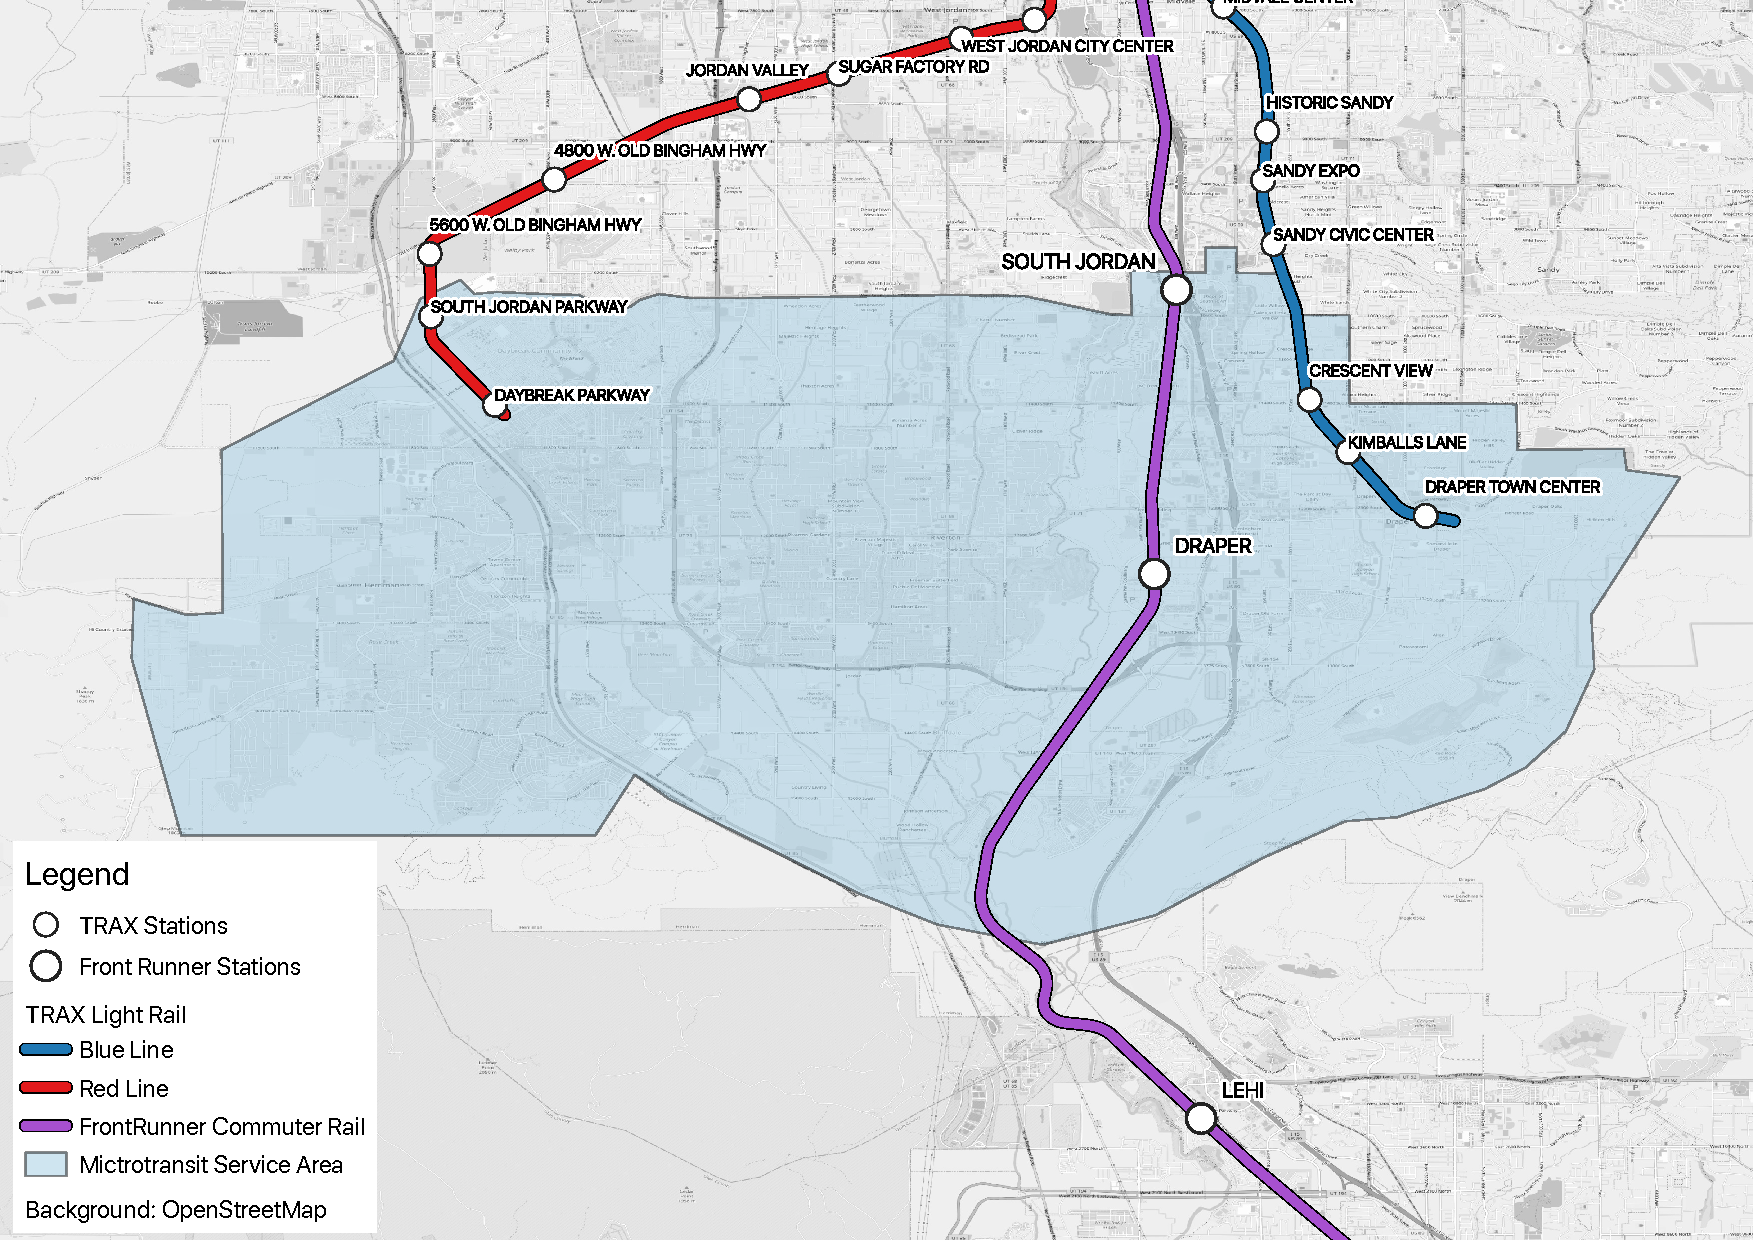
\includegraphics[width = \textwidth]{service_area.pdf}
    \caption{UTA on-demand microtransit service area. Image by the authors, using data from Utah AGRC and OpenStreetMap.}
    \label{fig:via-map}
\end{figure}

In establishing the on-demand microtransit service UTA partnered with Via, a commercial mobility provider with new and ongoing operations in several US cities. Passengers request rides using the VIA mobile application or calling a designated service line and await the vehicle at a pickup point near to their origin. Passengers share rides based on the availability of vehicles and the compatibility of paths, as determined by algorithms embedded in the VIA service. The vehicle will drop the passenger off near their destination or at TRAX or FrontRunner stations; both the pickup and drop-off points must lie within the service area shown in Figure \ref{fig:via-map}. The regular adult one-way fare is \$2.50 and includes a limited transfer to the UTA fixed route transit system. By the end of February 2020, the microtransit system was carrying about 316 passenger trips per weekday with an average wait time of 11 minutes per trip \citep{uta2020}.



\subsection{Survey Design}
UTA’s primary goal in executing this survey was to understand the effectiveness of its marketing campaign to raise awareness and information of the new service. This survey also provided an opportunity to inform additional riders and to evaluate rider perceptions and characteristics both before and immediately after the service launch. As such the survey was administered in two tranches. The first tranche was conducted on November 6th, 13th, and 14th of 2019 through on-platform intercept interviews at the Draper and South Jordan FrontRunner stations as well as the Draper Town Center TRAX station. The second tranche was collected on several weekdays between January 10th and March 4th, 2020, and was collected through on-platform intercept interviews at the same stations in addition to the Daybreak Parkway TRAX station and at designated microtransit pick-up points near the aforementioned rail stations; a limited number of interviews were also conducted on board the microtransit vehicles. Interviews were conducted throughout the day, but with a focus on the PM peak commute period. The number of interviews conducted during each time period for each tranche is shown in Table \ref{tab:survey-times}.

\begin{table}[ht]
    \centering
    \caption{Surveys Collected by Time of Day}
    \label{tab:survey-times}
    \begin{tabular}{lcc}
    \toprule
    Day Period           & Before   Launch & After   Launch \\
    \midrule
    AM (6-10)            & 7               & 6              \\
    Mid-Day (10-4)       & 13              & 26             \\
    PM (4-7)             & 33              & 43             \\
    Evening (7-Midnight) & 2               & 0              \\
    TOTAL                & 55              & 75            \\
    \bottomrule
    \end{tabular}
\end{table}

The surveys were administered via electronic tablet using a questionnaire developed in a web-based survey software. The survey questions were developed with the help of UTA staff and an external consulting team. The relevant variables and source questions for this study are shown in Table \ref{tab:survey-summary}, in the order in which the questions were asked. After asking the respondent about their awareness of the system, the interviewer would give a brief explanation of the service before asking about the respondent’s likeliness to use the system. The questionnaire for the second tranche included additional questions that were identified as being important after the first tranche was collected; for example, the questions about income and household size were added between the tranches. Further, questions in the second tranche for respondents on train platforms and either at or on board the microtransit service had slightly different wording to reflect the separate contexts. There was also a set of questions requesting general feedback on the UTA service that is not included in this study.

\begin{table}[ht]
\renewcommand{\arraystretch}{1.5}
    \centering
    \caption{Survey Questionnaire Summary}
    \label{tab:survey-summary}
\begin{tabular}{l p{0.4\textwidth}p{0.3\textwidth}}
\toprule
Variable          & Question Text                                                                                    & Response Type                                     \\
\midrule
Frequency         & How often do you ride UTA?                                                                       & Multiple choice with days   per week              \\
Purpose           & Where are you headed today?                                                                      & Multiple choice with   purposes plus text "other" \\
Access Mode       & How did you travel to your   UTA stop/station today?                                             & Multiple choice with modes   plus text "other"    \\
Awareness         & Had you heard about UTA On   Demand before today?                                                & Yes / No                                          \\
Likeliness        & How likely are you to   download the VIA app and use UTA On Demand?                              & Likert scale with five   "likely" levels          \\
Why Likely        & Why did you choose that   ranking?                                                               & Text response                                     \\
Use Purpose       & What types of trips do you   think you could use it for?                                         & Multiple choice with   purposes plus text "other" \\
Auto Availability & How many vehicles (cars,   trucks or motorcycles) are available in your household?               & Multiple choice with 0   through 4+               \\
Household Size    & Including you, how many   people live in your household?                                         & Numeric                                           \\
Race              & What is your race /   ethnicity?                                                                 & Mutiple choice allowing   multiple selection      \\
Income            & Which of the following BEST   describes your TOTAL ANNUAL HOUSEHOLD INCOME in 2019 before taxes? & Multiple choice in ranges                         \\
Smartphone        & Do you have a smartphone?                                                                        & Yes / No                                          \\
Age               & What is your age?                                                                                & Multiple choice in ranges    \\
\bottomrule
\end{tabular}
\end{table}

%%%%%%%%%%%%%%%%%%%%%%%%%%%%%%%%%%%%%%%%%%
\section{Results}

The surveyors conducted 55 interviews in the first tranche and 75 in the second tranche; the second tranche consisted of 58 interviews on rail transit platforms and 17 interviews on the mictrotransit vehicles or at the microtransit pick-up point adjacent to the rail stations. A summary of the survey respondents in each tranche is given in Table \ref{tab:survey-respondents}; as outlined in the Methodology section, the decision to include income level in the survey was made between the tranches and therefore the “Before” tranche contains no income information. The number of respondents who declined to answer the other demographic questions is also relatively high.

\begin{table}[ht]
    \centering
    \caption{Demographic Characteristics of Survey Respondents}
    \label{tab:survey-respondents}
 \renewcommand{\arraystretch}{1.5}

\begin{tabular}{@{}lcc@{}}
\toprule
                   & Before (n   = 55) & After (n   = 75) \\ \midrule
\emph{Smartphone}         &                   &                  \\
\quad Yes                & 42                & 48               \\
\quad No                 & 3                 & 2                \\
\quad No Response        & 10 (18.18\%)      & 25 (33.33\%)     \\
\emph{Auto Availability} &                   &                  \\
\quad 0                  & 0                 & 4                \\
\quad 1                  & 18                & 19               \\
\quad 2                  & 13                & 18               \\
\quad 3                  & 8                 & 8                \\
\quad 4+                 & 3                 & 5                \\
\quad No Response        & 13 (23.64\%)      & 21 (28.00\%)     \\
\emph{Income}             &                   &                  \\
\quad Less than \$44,999 & 0                 & 8                \\
\quad \$45,000 - \$99,999  & 0                 & 17               \\
\quad Over \$100k        & 0                 & 17               \\
\quad No Response        & 55 (100.00\%)     & 31 (41.33\%)     \\
\emph{Age}                &                   &                  \\
\quad Under 18           & 0                 & 3                \\
\quad 18-24              & 12                & 8                \\
\quad 25-44              & 24                & 28               \\
\quad 45-64              & 9                 & 10               \\
\quad Over 65            & 0                 & 1                \\
\quad No Response        & 10 (18.18\%)      & 25 (33.33\%)     \\ \bottomrule
\end{tabular}
\end{table}

A primary motivation for the survey was to understand awareness of the microtransit service among UTA transit riders. In the “Before” tranche, only 6 of the 55 respondents (11\%) stated they had previously heard of the system. Of the 58 interviews in the “After” tranche not conducted on the microtransit service, 34 (59\%) had previously heard of the service. This increase in general awareness of the system indicates both that the UTA marketing efforts were effective, and also that the responses to the subsequent question of likeliness to use the service are based in some level of understanding.

Figure \ref{fig:likelihood} shows the reported likelihood of survey respondents to download the necessary application and use the microtransit service, separated by access mode. Respondents who were already using the service selected “5: Extremely Likely.” The first result of this analysis is that there appears to be a polarization in opinions after the service commenced operations. Although there are some strong feelings against and for the service in the “Before” tranche, the neutral opinions have comparatively disappeared in the “After” tranche. This likely reflects the increasing awareness of the service discussed above and a hardening of engrained or newly learned habits. It is important also to stress that the question will not necessarily elicit an opinion as to whether the service should exist, merely whether the particular respondent is willing to use it.

The sample is too small to conduct meaningful statistical inference on the role that access mode plays in these opinions, but some discussion of these observations is still worthwhile. The apparent turning of bicycle users against the service is likely statistical noise, though it should also be noted that the “After” tranche was collected in January and February, when Utah is typically cold with snow on the ground. Perhaps individuals who are still cycling at those times will persist in doing so. It is also interesting to note that there appears to be little overall correlation between access mode and expressed willingness to use the service, unless the UTA On Demand service attracts people who would not have used the service otherwise. Of these individuals who responded to a question about their hypothetical alternative mode, four reported that they would have used a Transportation Network Company (TNC; e.g. Uber, Lyft, etc.), two would have used regular UTA services, two would have driven to the transit station, one would have walked, and one would not have used transit at all. Additionally, the text responses to the access mode question in the “before” tranche revealed a number of individuals who used a TNC to access the system. This supplies anecdotal evidence that microtransit is competing more against commercial TNC offerings than against conventional transit services.

\begin{figure}
    \centering
    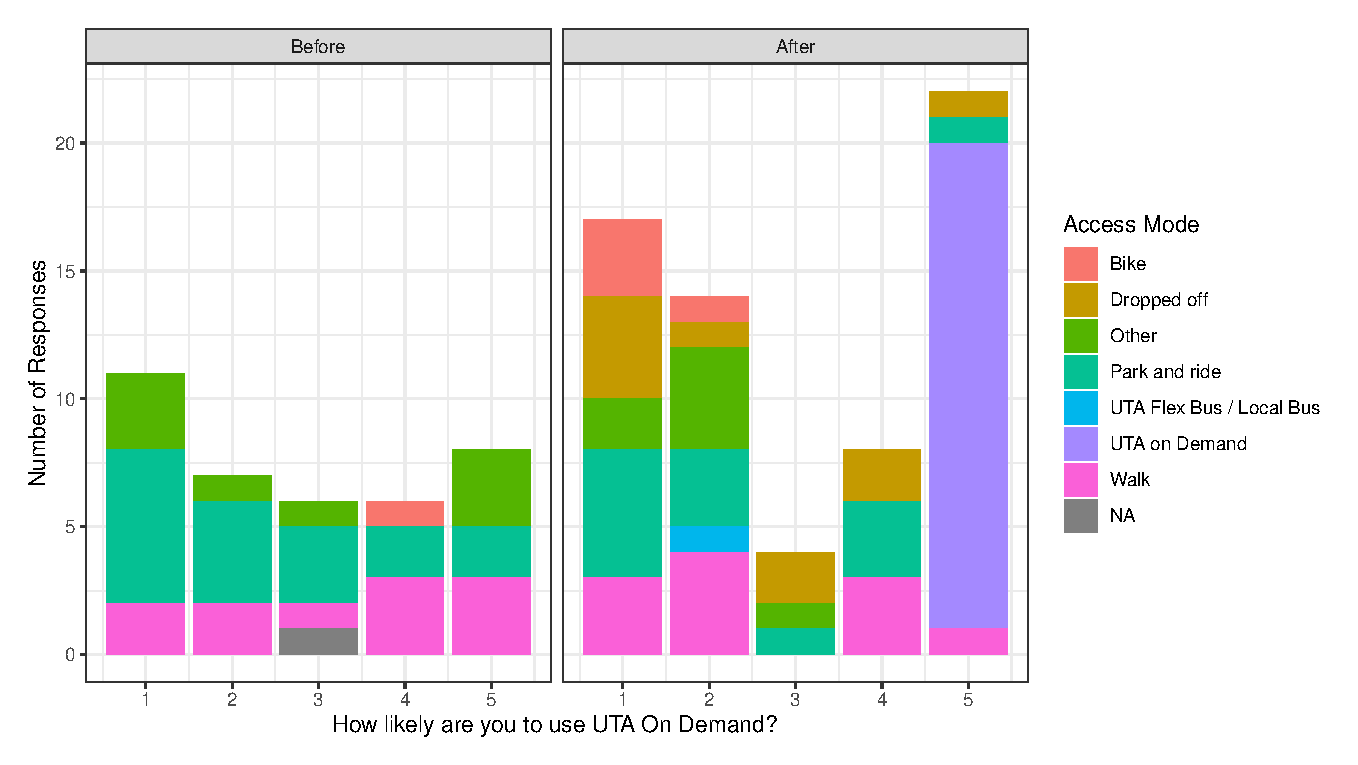
\includegraphics[width = \textwidth]{access_mode.eps}
    \caption{Reported likelihood of using microtransit by transit access mode.}
    \label{fig:likelihood}
\end{figure}

The next consideration is whether the expressed or observed likeliness to use the microtransit service is related to the demographic characteristics of the respondents. Noting the low response rate to many of the demographic questions (see Table \ref{tab:survey-summary}), it is not possible to construct a model that would predict the likeliness score as a function of these characteristics in combination. It is still valuable, however, to consider how the observed distribution of these characteristics differs between individuals who are or are not likely to use the service. These distributions are shown in Table \ref{tab:likeliness}, along with the result of a two-sided Fisher exact test of independence between the indicated characteristic distribution and the three-category likeliness response. In this test the null hypothesis is that the two distributions are independent with the alternative being there is some dependence between the characteristic and the response. A $p$-value less than a given critical threshold indicates that the null hypothesis has a low probability and should be rejected. A conventional value of the critical value is $\alpha=0.05$, though given the small sample sizes in this survey other critical values may be suggestive of the need for future evaluation.

\begin{table}[ht]
    \centering
     \renewcommand{\arraystretch}{1.5}
    \caption{Distribution of Rider Characteristics by Reported Likeliness}
    \label{tab:likeliness}
\begin{tabular}{@{}lccc@{}}
\toprule
                   & Not Likely (1 and 2) & Neutral (3) & Likely (4 and 5) \\
\midrule
\multicolumn{4}{l}{\emph{Smartphone} ($p_F = 0.563$ on 2 degrees of freedom)}\\
\quad Yes                & 41 (95\%)            & 8 (89\%)    & 30 (97\%)        \\
\quad No                 & 2 (5\%)              & 1 (11\%)    & 1 (3\%)          \\
\multicolumn{4}{l}{\emph{Household Size} ($p_F = 0.207$ on 6 degrees of freedom)}\\
\quad 1                  & 2 (7\%)              & 0 (0\%)     & 2 (14\%)         \\
\quad 2                  & 8 (29\%)             & 0 (0\%)     & 1 (7\%)          \\
\quad 3                  & 4 (14\%)             & 1 (25\%)    & 0 (0\%)          \\
\quad 4+                 & 14 (50\%)            & 3 (75\%)    & 11 (79\%)        \\
\multicolumn{4}{l}{\emph{Auto Availability} ($p_F = 0.659$ on 8 degrees of freedom)}\\
\quad 0                  & 1 (2\%)              & 0 (0\%)     & 3 (10\%)         \\
\quad 1                  & 22 (49\%)            & 3 (33\%)    & 10 (33\%)        \\
\quad 2                  & 12 (27\%)            & 3 (33\%)    & 9 (30\%)         \\
\quad 3                  & 7 (16\%)             & 1 (11\%)    & 5 (17\%)         \\
\quad 4+                 & 3 (7\%)              & 2 (22\%)    & 3 (10\%)         \\
\multicolumn{4}{l}{\emph{Income} ($p_F = 0.687$ on 4 degrees of freedom)}\\
\quad Less than \$44,999 & 4 (17\%)             & 1 (33\%)    & 3 (21\%)         \\
\quad $45,000 - $99,999  & 10 (44\%)            & 2 (67\%)    & 5 (36\%)         \\
\quad Over \$100k        & 9 (39\%)             & 0 (0\%)     & 6 (43\%)         \\
\quad Under 18           & 1 (2\%)              & 2 (20\%)    & 0 (0\%)          \\
\multicolumn{4}{l}{\emph{Age} ($p_F = 0.00364^*$ on 8 degrees of freedom)}\\
\quad 18-24              & 7 (16\%)             & 2 (20\%)    & 9 (31\%)         \\
\quad 25-44              & 28 (64\%)            & 1 (10\%)    & 17 (59\%)        \\
\quad 45-64              & 7 (16\%)             & 5 (50\%)    & 3 (10\%)         \\
\quad Over 65            & 1 (2\%)              & 0 (0\%)     & 0 (0\%)         \\
\bottomrule
\multicolumn{4}{l}{$^*$ indicates $p$-value less than 0.05}

\end{tabular}
\end{table}


Smartphone use appears to not be a contributing factor in the likeliness of using microtransit, as almost all respondents use a smartphone regardless of their reported likeliness. We also fail to reject the null hypothesis of independence between the likeliness to use microtransit and both auto availability and household income. The joint distribution of reported likeliness and household size suggests there could be some dependence, with members of smaller households more frequently expressing reluctance to use microtransit. This finding, if it could be verified, would be somewhat counter to the \emph{a priori} expectations of UTA. A Fisher test of independence between these household size and expressed likeliness still fails to conclusively reject the null hypothesis but given the small sample size and counter-intuitive results, future investigation is warranted. This is particularly true given that automobile availability and household size go hand-in-hand: a household with more individuals, particularly driving-age individuals, will be more constrained in their driving behavior even with multiple household automobiles. Considering these two variables together will be important for future research but cannot be attempted here.

A clear statistical result is shown, however, between the reported willingness to use microtransit and the age of the respondent. This significant result persists when we recombine the age categories as well as discard neutral responses. Table \ref{tab:age-difference} shows the differences between the observed values in the joint distribution of these two variables and the expected values based on the marginal distributions were the two variables to be completely independent. The largest differences occur in three noticeable places. First, individuals in the 18-24 years old category are more likely to express willingness to use microtransit. Second, individuals between 45 and 64 are more likely to express a neutral opinion than a positive or strictly unlikely one. Finally, individuals between 25 and 44 are – perhaps surprisingly – substantially more likely to express a negative opinion than a neutral one; these individuals are also modestly more likely than expected to express positive willingness to use transit.

\begin{table}[ht]
    \centering
         \renewcommand{\arraystretch}{1.5}
    \caption{Difference of Observed and Expected Frequencies for Age and Likeliness}
    \label{tab:age-difference}
    \begin{tabular}{@{}lccc@{}}
\toprule
Age      & Not Likely & Neutral & Likely \\
\midrule
Under 18 & – 0.59     & 1.64    & – 1.05 \\
18-24    & – 2.54     & – 0.17  & 2.71   \\
25-44    & 3.61       & – 4.54  & 0.93   \\
45-64    & –0.95      & 3.19    & – 2.24 \\
Over 65  & 0.47       & – 0.12  & – 0.35\\
\bottomrule
\end{tabular}
\end{table}

%%%%%%%%%%%%%%%%%%%%%%%%%%%%%%%%%%%%%%%%%%
\section{Discussion}
We readily acknowledge several limitations of this study, particularly in the survey design and methodology. The interviews were conducted as a convenience sample rather than with a rigorous sampling strategy, with the statistical caveats resulting from that design decision. The sample is also too small to have substantial statistical power, particularly in statistics calculated on multiple grouping dimensions. Finally, the survey collected self-reported responses with no verification or validation of any kind.

Most survey responses were collected on fixed rail transit station platforms. Passengers waiting for UTA trains were expected to be both more available to respond to survey questions, as well as more likely to use the microtransit service than the general population. Additionally, UTA is interested in supporting its fixed rail transit investments in the service area. There is, however, no requirement that microtransit passengers use other UTA services; data supplied by the microtransit provider but not included in this study suggest that only 58\% percent of microtransit trips began or ended within 500 feet of a UTA rail transit station. This population might have preferences or patterns that either match or contradict the initial findings of this research.

In discussing the responses to the question of what mode microtransit passengers would have used were the service not available, we suggested there is anecdotal evidence that commercial TNC rides are the primary competition. There are still questions, however, of how use of this service might affect conventional transit services. Table \ref{tab:uta-ridership} shows the average weekday ridership during November, December, and January for the period the microtransit service was operating as well as the same three months in the two prior years \citet{uta2020boardings}. Total system ridership was remarkably stable during these three periods. The microtransit service area – in this case defined by ridership on routes F514, 218, 526, F504, F518, F534, F546, and F547 – was declining before the microtransit service began, though the decline accelerated during the first three months of the service’s operation. By comparison, the microtransit service carried approximately 316 passengers per day during its first three months, more than compensating for the recent observed decline in transit ridership were this to be identified as a major contributing factor.

\begin{table}[ht]
    \centering
    \renewcommand{\arraystretch}{1.5}
    \caption{Average Weekday Ridership, November through January}
    \label{tab:uta-ridership}
    \begin{tabular}{@{}lcccc@{}}
\toprule
          & \multicolumn{2}{c}{All   Other UTA Services} & \multicolumn{2}{c}{Microtransit   Service Region} \\
          \cmidrule(l){2-3} \cmidrule(l){4-5}
Year      & Average   Weekday Riders    & \%   Change    & Average   Weekday Riders    & \%   Change\\
\midrule
2019-2018 & 147,410                     &                & 1,179                       &            \\
2018-2019 & 146,743                     & –   0.452\%    & 1,125                       & –   4.61\% \\
2019-2020 & 147,010                     & 0.182          & 970                         & –   13.7\% \\
\bottomrule
\end{tabular}
\end{table}

Another limitation of these findings that is particularly relevant is the onset of the COVID-19 pandemic. Government-imposed shutdowns and voluntary work stoppages related to the pandemic did not begin in Utah until the week of March 15th, after data collection for this project had completed. As such, the survey responses are likely unaffected by changes in behavior related to the pandemic. However, the pandemic has drastically affected the subsequent operations of both UTA and Via and is likely to change many of the stated behaviors and attitudes reported in this study. Many findings of this study will need to be reconsidered should “normal” operations resume.

%%%%%%%%%%%%%%%%%%%%%%%%%%%%%%%%%%%%%%%%%%
\subsection{Conclusion}

Microtransit services are regularly put forward as means to support last-mile / first-mile trips on fixed route transit systems, and several such systems have been deployed in the recent past. This paper presented initial findings from a quick response survey aimed at learning who was most willing to use the new service within weeks of the system launch. These initial findings suggest first that younger adults are most willing to consider using microtransit services, and that these services compete most directly with commercial TNC ridehail offerings rather than conventional transit.

Transit passenger intercept surveys are an important method to determine who is and who is not using a microtransit service, paired with demographic characteristics and trip purpose information. To understand the rider characteristics and trip purposes specifically of microtransit users, by contrast, better survey methods are needed. In particular, a survey pushed through the smartphone application used by the passengers would help in reaching a considerably larger sample. It would also be theoretically possible in that case for the researchers to pair the survey responses with actual observed trip patterns for distinct users including origin, destination, and route GPS points, regularity of use and variance in use patterns, and many other data variables. Obtaining these data and conducting responsible research with them should be a priority for the service operators and their agency partners.


%%%%%%%%%%%%%%%%%%%%%%%%%%%%%%%%%%%%%%%%%%
\vspace{6pt}

%%%%%%%%%%%%%%%%%%%%%%%%%%%%%%%%%%%%%%%%%%
\authorcontributions{Data curation, Christian Hunter, Austin Martinez and Elizabeth Smith; Investigation, Christian Hunter, Austin Martinez and Elizabeth Smith; Methodology, Christian Hunter, Austin Martinez and Elizabeth Smith; Project administration, Gregory S. Macfarlane; Supervision, Gregory S. Macfarlane; Writing -- original draft, Gregory S. Macfarlane; Writing -- review \& editing, Gregory S. Macfarlane, Christian Hunter and Elizabeth Smith}

%%%%%%%%%%%%%%%%%%%%%%%%%%%%%%%%%%%%%%%%%%
\funding{This research received no external funding.}

%%%%%%%%%%%%%%%%%%%%%%%%%%%%%%%%%%%%%%%%%%
\acknowledgments{This project was sponsored by UTA through the BYU Civil Engineering Capstone Program. The authors would like to thank Jaron Robertson and Shaina Quinn of UTA and Sahar Shirazi and Kenny Ferrel of WSP for oversight and input throughout the project.}

%%%%%%%%%%%%%%%%%%%%%%%%%%%%%%%%%%%%%%%%%%
\conflictsofinterest{The authors declare no conflict of interest.}

%%%%%%%%%%%%%%%%%%%%%%%%%%%%%%%%%%%%%%%%%%
%% optional
\abbreviations{The following abbreviations are used in this manuscript:\\

\noindent
\begin{tabular}{@{}ll}
TNC & Transportation Network Company, e.g. Uber, Lyft\\
UTA & Utah Transit Authority\\
\end{tabular}}

%%%%%%%%%%%%%%%%%%%%%%%%%%%%%%%%%%%%%%%%%%
% Citations and References in Supplementary files are permitted provided that they also appear in the reference list here.

%=====================================
% References, variant A: internal bibliography
%=====================================
%\reftitle{References}
%\begin{thebibliography}{999}
% Reference 1
%\bibitem[Author1(year)]{ref-journal}
%Author1, T. The title of the cited article. {\em Journal Abbreviation} {\bf 2008}, {\em 10}, 142--149.
% Reference 2
%\bibitem[Author2(year)]{ref-book}
%Author2, L. The title of the cited contribution. In {\em The Book Title}; Editor1, F., Editor2, A., Eds.; Publishing House: City, Country, 2007; pp. 32--58.
%\end{thebibliography}

% The following MDPI journals use author-date citation: Arts, Econometrics, Economies, Genealogy, Humanities, IJFS, JRFM, Laws, Religions, Risks, Social Sciences. For those journals, please follow the formatting guidelines on http://www.mdpi.com/authors/references
% To cite two works by the same author: \citeauthor{ref-journal-1a} (\citeyear{ref-journal-1a}, \citeyear{ref-journal-1b}). This produces: Whittaker (1967, 1975)
% To cite two works by the same author with specific pages: \citeauthor{ref-journal-3a} (\citeyear{ref-journal-3a}, p. 328; \citeyear{ref-journal-3b}, p.475). This produces: Wong (1999, p. 328; 2000, p. 475)

%=====================================
% References, variant B: external bibliography
%=====================================
\externalbibliography{yes}
\bibliography{citations}

%%%%%%%%%%%%%%%%%%%%%%%%%%%%%%%%%%%%%%%%%%
%% optional

%% for journal Sci
%\reviewreports{\\
%Reviewer 1 comments and authors’ response\\
%Reviewer 2 comments and authors’ response\\
%Reviewer 3 comments and authors’ response
%}

%%%%%%%%%%%%%%%%%%%%%%%%%%%%%%%%%%%%%%%%%%
\end{document}
